\cohead{\Large\textbf{Schnittstellen und Schnittpunkte}}
\fakesubsection{Schnittstellen und Schnittpunkte}
Erinnerung: In der Mathematik unterscheidet man grundsätzlich zwischen Stellen und Punkten. Stellen sind x-Werte während Punkte einen x-Wert und einen y-Wert haben. Die Schnittpunkte zweier Funktionen $f(x)$ und $g(x)$ sind alle Punkte, in denen sich die Schaubilder schneiden. Um die Schnittstellen zu erhalten, muss man die Funktionen gleichsetzen:
\begin{tcolorbox}\centering
	$\textcolor{loestc}{f(x)=g(x)}$
\end{tcolorbox}
\begin{minipage}{0.49\textwidth}
	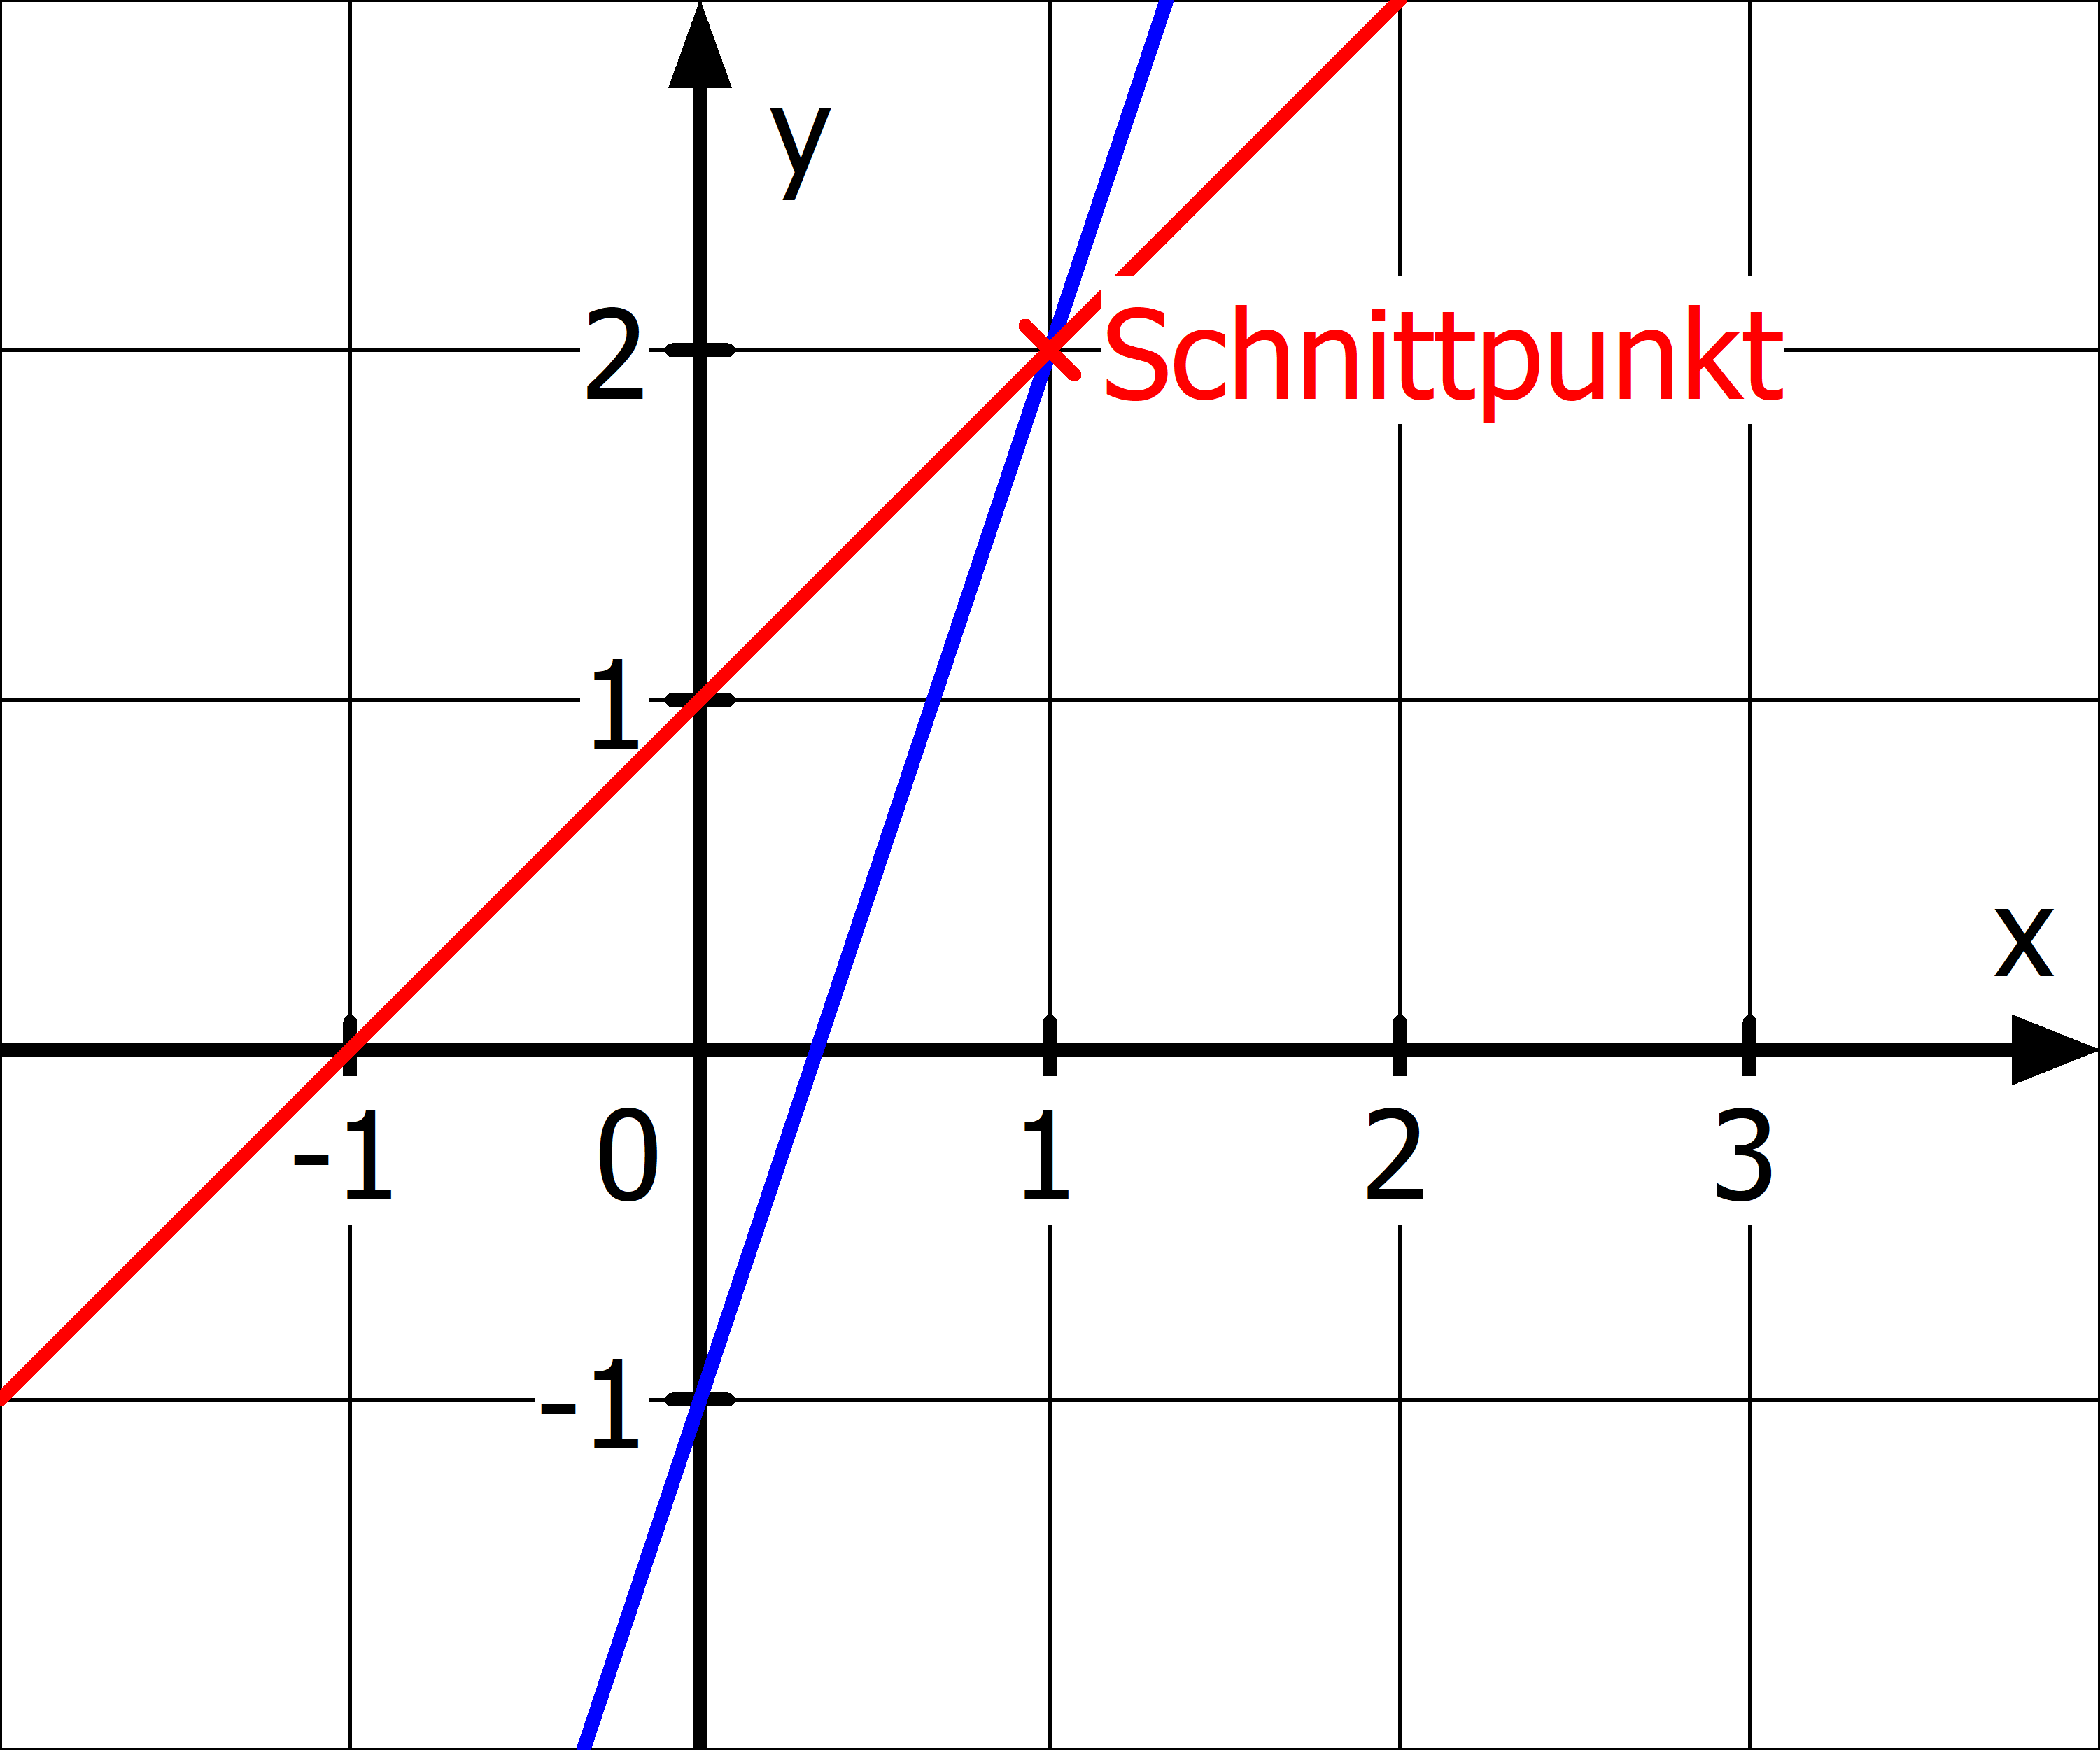
\includegraphics[width=.95\textwidth]{\linFkt/pics/schnittpunkt.png}
\end{minipage}
\begin{minipage}{0.49\textwidth}
	Im nebenstehenden Beispiel sind die Schaubilder der Funktionen $\textcolor{red}{f(x)=x+1}$ und $\textcolor{blue}{g(x)=3x-1}$ gezeichnet. Der Schnittpunkt lässt sich wie folgt berechnen:
	\begin{align*}
		\textcolor{red}{f(x)}&=\textcolor{blue}{g(x)}\\
		\textcolor{red}{x+1}&=\textcolor{blue}{3x-1}\ \rvert -3x-1\\
		-2x&=-2\ \rvert \cdot\left(-\tfrac{1}{2}\right)\\
		x&=1
	\end{align*}
\end{minipage}\smallskip\\
Die Schnittstelle ist also $\textcolor{ForestGreen}{x=1}$. Um die y-Koordinate zu erhalten, setzt man $\textcolor{ForestGreen}{x=1}$ entweder in $\textcolor{red}{f(x)}$ oder $\textcolor{blue}{g(x)}$ ein. Zur Demonstration setzen wir die Schnittstelle in beide Funktionen ein:
\begin{align*}
	\textcolor{red}{f(}\textcolor{ForestGreen}{1}\textcolor{red}{)}&=\textcolor{red}{\textcolor{ForestGreen}{1}+1}=\textcolor{YellowOrange}{2}\\
	\textcolor{blue}{g(}\textcolor{ForestGreen}{1}\textcolor{blue}{)}&=\textcolor{blue}{3\cdot \textcolor{ForestGreen}{1}-1}=\textcolor{YellowOrange}{2}
\end{align*}
Der Schnittpunkt liegt also bei $P\left(\textcolor{ForestGreen}{1}\lvert\textcolor{YellowOrange}{2}\right)$.
\begin{Exercise}[title={Bestimme jeweils den Schnittpunkt}, label=schnittpunktA1]\\
	\begin{minipage}{0.5\textwidth}
		\begin{enumerate}[label=\alph*)]
			\item $f_1(x)=x-1$ und $g_1(x)=-x+3$
			\item $f_2(x)=-2x+4$ und $g_2(x)=0,5x-1$
			\item $f_3(x)=\frac{3}{2}x+\frac{1}{2}$ und $g_3(x)=4x$
		\end{enumerate}
	\end{minipage}
	\begin{minipage}{0.5\textwidth}
		\begin{enumerate}[label=\alph*)]
			\setcounter{enumi}{3}
			\item $f_4(x)=\frac{4}{5}x+\frac{2}{5}$ und $g_4(x)=-\frac{2}{5}x$
			\item $f_5(x)=-\frac{2}{3}x-15$ und $g_5(x)=3x-\frac{5}{4}$
			\item $f_6(x)=-\frac{5}{8}x$ und $g_6(x)=-\frac{3}{2}x+\frac{1}{2}$
		\end{enumerate}
	\end{minipage}
\end{Exercise}\vspace{.5cm}
\begin{Answer}[ref=schnittpunktA1]\\
	\begin{minipage}{0.5\textwidth}
		\begin{enumerate}[label=\alph*)]
			\item $P_1\left(2\vert 1\right)$
			\item $P_2\left(2\vert 0\right)$
			\item $P_3\left(\frac{1}{5}\vert \frac{4}{5}\right)$
		\end{enumerate}
	\end{minipage}
	\begin{minipage}{0.5\textwidth}
		\begin{enumerate}[label=\alph*)]
			\setcounter{enumi}{3}
			\item $P_4\left(-\frac{1}{3}\vert -\frac{2}{15}\right)$
			\item $P_5\left(-\frac{15}{4}\vert -\frac{25}{2}\right)$
			\item $P_6\left(\frac{4}{7}\vert -\frac{5}{14}\right)$
		\end{enumerate}
	\end{minipage}
\end{Answer}